\chapter{Results and Analysis}

This chapter presents the final experimental results of the traffic sign classification system. We evaluate the performance of the proposed pipeline across two backbone architectures and two Support Vector Machine configurations.

\section{Evaluation Metrics for Classification}
To provide a rigorous assessment of the traffic sign recognition system, we utilize four fundamental metrics derived from the confusion matrix (True Positives $TP$, True Negatives $TN$, False Positives $FP$, and False Negatives $FN$):

\begin{enumerate}
    \item \textbf{Accuracy ($Acc$):} The proportion of total number of correct predictions (both True Positives and True Negatives) among the total number of cases examined. It provides a general measure of how often the classifier is correct.
    \begin{equation}
        \text{Accuracy} = \frac{TP + TN}{TP + TN + FP + FN}
    \end{equation}

    \item \textbf{Precision ($P$):} The ratio of correctly predicted positive observations to the total predicted positives. It represents the model's ability not to label a negative sample as positive.
    \begin{equation}
        \text{Precision} = \frac{TP}{TP + FP}
    \end{equation}
    
    \item \textbf{Recall ($R$):} The ratio of correctly predicted positive observations to all observations in the actual class. It measures the model's ability to find all positive samples.
    \begin{equation}
        \text{Recall} = \frac{TP}{TP + FN}
    \end{equation}
    
    \item \textbf{F1-Score ($F1$):} The harmonic mean of Precision and Recall, providing a single metric that balances both concerns, especially useful for imbalanced datasets.
    \begin{equation}
        F1 = 2 \cdot \frac{\text{Precision} \cdot \text{Recall}}{\text{Precision} + \text{Recall}}
    \end{equation}
\end{enumerate}

\section{Overall Classification Performance}
The system's effectiveness is measured by its top-1 accuracy on the 20\% test set (stratified split). Table \ref{tab:final_acc} summarizes the comparative performance, highlighting the impact of feature extraction quality and kernel selection.

\begin{table}[H]
    \centering
    \caption{Final Classification Accuracy Comparison}
    \label{tab:final_acc}
    \begin{tabular}{lccc}
        \toprule
        \textbf{Extractor} & \textbf{SGD-SVM (Linear)} & \textbf{RBF-SVM (Non-linear)} & \textbf{Improvement ($\Delta$)} \\
        \midrule
        ResNet50 & 87.29\% & 93.46\% & +6.17\% \\
        InceptionV3 & 88.31\% & \textbf{97.24\%} & +8.93\% \\
        \bottomrule
    \end{tabular}
\end{table}

The empirical results show a consistent superiority of the \textbf{RBF-SVM} across both architectures. Notably, the combination of \textbf{InceptionV3} and the \textbf{RBF kernel} yielded the highest accuracy of \textbf{97.24\%}.

\section{Comparative Performance Analysis}
To better understand the strengths of the different SVM configurations, we analyze the classification metrics for each class across both architectures. 

\subsection{InceptionV3 Feature Performance}
We first focus on the InceptionV3 features as they provided the best overall baseline.

\begin{table}[H]
    \centering
    \caption{InceptionV3 Performance: SGD-SVM (Linear) vs. RBF-SVM (Non-linear)}
    \label{tab:metrics_comparison}
    \begin{tabular}{lcccccc}
        \toprule
        & \multicolumn{3}{c}{\textbf{SGD-SVM (Linear)}} & \multicolumn{3}{c}{\textbf{RBF-SVM (Non-linear)}} \\
        \cmidrule(lr){2-4} \cmidrule(lr){5-7}
        \textbf{Class ID} & \textbf{Precision} & \textbf{Recall} & \textbf{F1} & \textbf{Precision} & \textbf{Recall} & \textbf{F1} \\
        \midrule
        Class 0 & 0.69 & 0.74 & 0.71 & \textbf{1.00} & \textbf{0.86} & \textbf{0.92} \\
        Class 1 & 0.85 & 0.87 & 0.86 & \textbf{0.96} & \textbf{0.99} & \textbf{0.97} \\
        Class 2 & 0.81 & 0.86 & 0.84 & \textbf{0.95} & \textbf{0.97} & \textbf{0.96} \\
        Class 3 & 0.86 & 0.85 & 0.85 & \textbf{0.96} & \textbf{0.95} & \textbf{0.96} \\
        Class 4 & 0.93 & 0.87 & 0.90 & \textbf{0.99} & \textbf{0.96} & \textbf{0.97} \\
        Class 5 & 0.89 & 0.82 & 0.85 & \textbf{0.99} & \textbf{0.96} & \textbf{0.98} \\
        Class 6 & 0.97 & 0.93 & 0.95 & \textbf{0.99} & \textbf{0.99} & \textbf{0.99} \\
        Class 7 & 0.94 & 0.93 & 0.94 & \textbf{0.98} & \textbf{0.98} & \textbf{0.98} \\
        Class 8 & 0.87 & 0.94 & 0.90 & \textbf{0.96} & \textbf{0.99} & \textbf{0.97} \\
        Class 9 & 0.97 & 0.97 & 0.97 & \textbf{1.00} & \textbf{0.99} & \textbf{0.99} \\
        \midrule
        \textbf{Accuracy} & \multicolumn{3}{c}{88.31\%} & \multicolumn{3}{c}{\textbf{97.24\%}} \\
        \bottomrule
    \end{tabular}
\end{table}

The data demonstrates that the RBF kernel provides a significant boost across all classes, particularly for Class 0, where precision increased from 0.69 to 1.00. This confirms that the RBF kernel successfully navigated the high-dimensional feature clusters that were not perfectly separable by a linear hyperplane.

\subsection{ResNet50 Feature Performance}
Similarly, we evaluate the ResNet50 features to confirm the consistency of the RBF kernel's advantages.

\begin{table}[H]
    \centering
    \caption{ResNet50 Performance: SGD-SVM (Linear) vs. RBF-SVM (Non-linear)}
    \label{tab:resnet_metrics_comparison}
    \begin{tabular}{lcccccc}
        \toprule
        & \multicolumn{3}{c}{\textbf{SGD-SVM (Linear)}} & \multicolumn{3}{c}{\textbf{RBF-SVM (Non-linear)}} \\
        \cmidrule(lr){2-4} \cmidrule(lr){5-7}
        \textbf{Class ID} & \textbf{Precision} & \textbf{Recall} & \textbf{F1} & \textbf{Precision} & \textbf{Recall} & \textbf{F1} \\
        \midrule
        Class 0 & 0.86 & 0.60 & 0.70 & \textbf{1.00} & \textbf{0.74} & \textbf{0.85} \\
        Class 1 & 0.85 & 0.88 & 0.86 & \textbf{0.86} & \textbf{0.95} & \textbf{0.90} \\
        Class 2 & 0.79 & 0.86 & 0.82 & \textbf{0.93} & \textbf{0.94} & \textbf{0.94} \\
        Class 3 & 0.86 & 0.83 & 0.85 & \textbf{0.94} & \textbf{0.92} & \textbf{0.93} \\
        Class 4 & 0.89 & 0.86 & 0.87 & \textbf{0.95} & \textbf{0.95} & \textbf{0.95} \\
        Class 5 & 0.84 & 0.86 & 0.85 & \textbf{0.92} & \textbf{0.93} & \textbf{0.92} \\
        Class 6 & 1.00 & 1.00 & 1.00 & \textbf{1.00} & 0.92 & 0.96 \\
        Class 7 & 0.93 & 0.89 & 0.91 & \textbf{0.97} & \textbf{0.92} & \textbf{0.94} \\
        Class 8 & 0.88 & 0.87 & 0.87 & \textbf{0.94} & \textbf{0.90} & \textbf{0.92} \\
        Class 9 & 0.99 & 0.95 & 0.97 & \textbf{1.00} & \textbf{0.97} & \textbf{0.98} \\
        \midrule
        \textbf{Accuracy} & \multicolumn{3}{c}{87.29\%} & \multicolumn{3}{c}{\textbf{93.46\%}} \\
        \bottomrule
    \end{tabular}
\end{table}

ResNet50 also shows substantial improvements, especially in Class 2, where the F1-Score jumped from 0.82 to 0.94 (+12\%). While the absolute performance is lower than InceptionV3, the trend of RBF-driven improvement remains identical.

\section{Confusion Matrix and Error Analysis}
To visually diagnose the model's behavior and identify specific inter-class confusions, we utilize the \texttt{confusion\_matrix} module. Figure \ref{fig:cm_comparison} provides a visual representation of these prediction patterns, with the matrices rendered using the \texttt{Seaborn} and \texttt{Matplotlib} libraries.

\begin{figure}[H]
    \centering
    \begin{subfigure}[b]{0.48\textwidth}
        \centering
        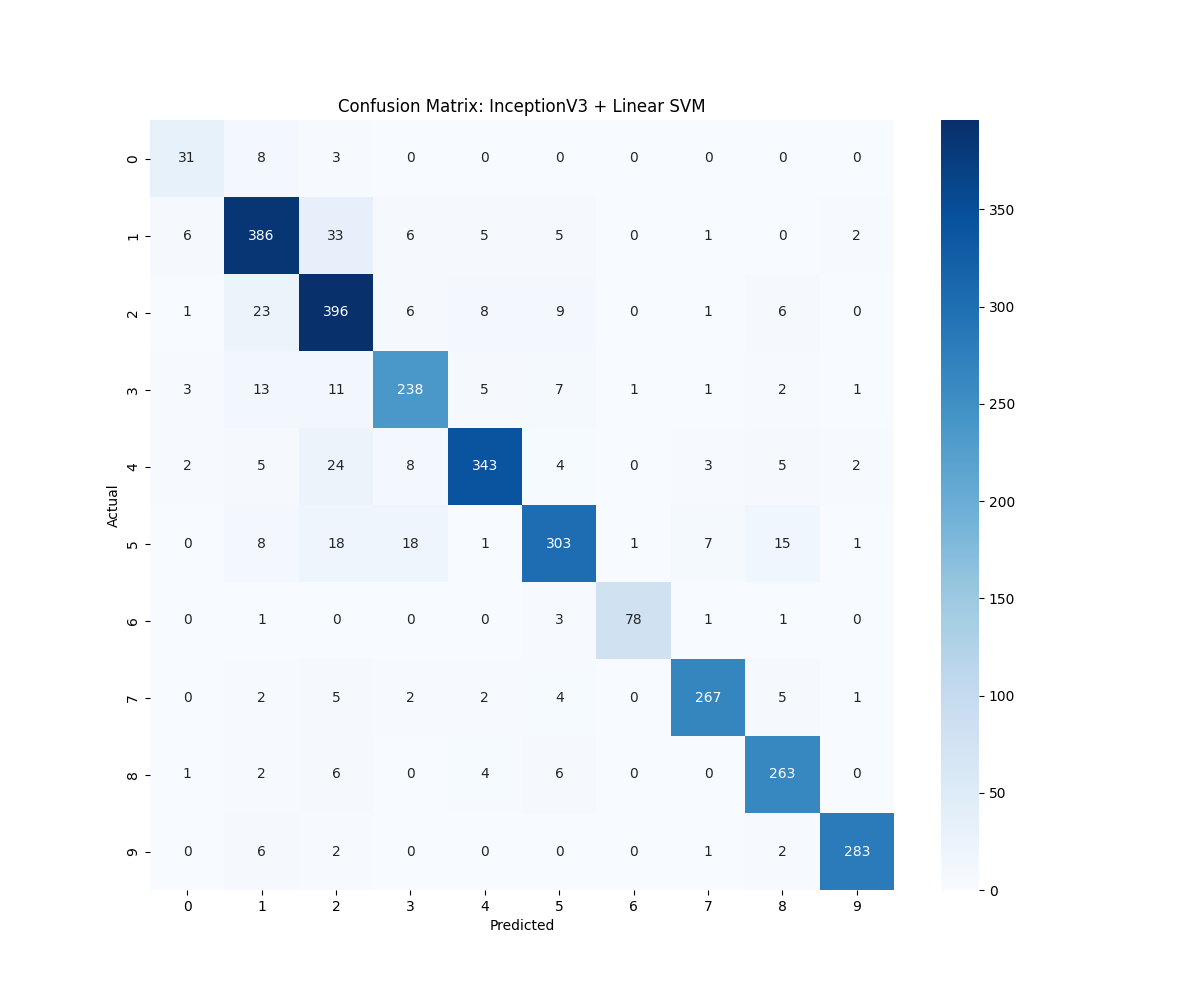
\includegraphics[width=\textwidth]{../reports/performance/inceptionv3_confusion_matrix.png}
        \caption{InceptionV3: SGD-SVM}
    \end{subfigure}
    \hfill
    \begin{subfigure}[b]{0.48\textwidth}
        \centering
        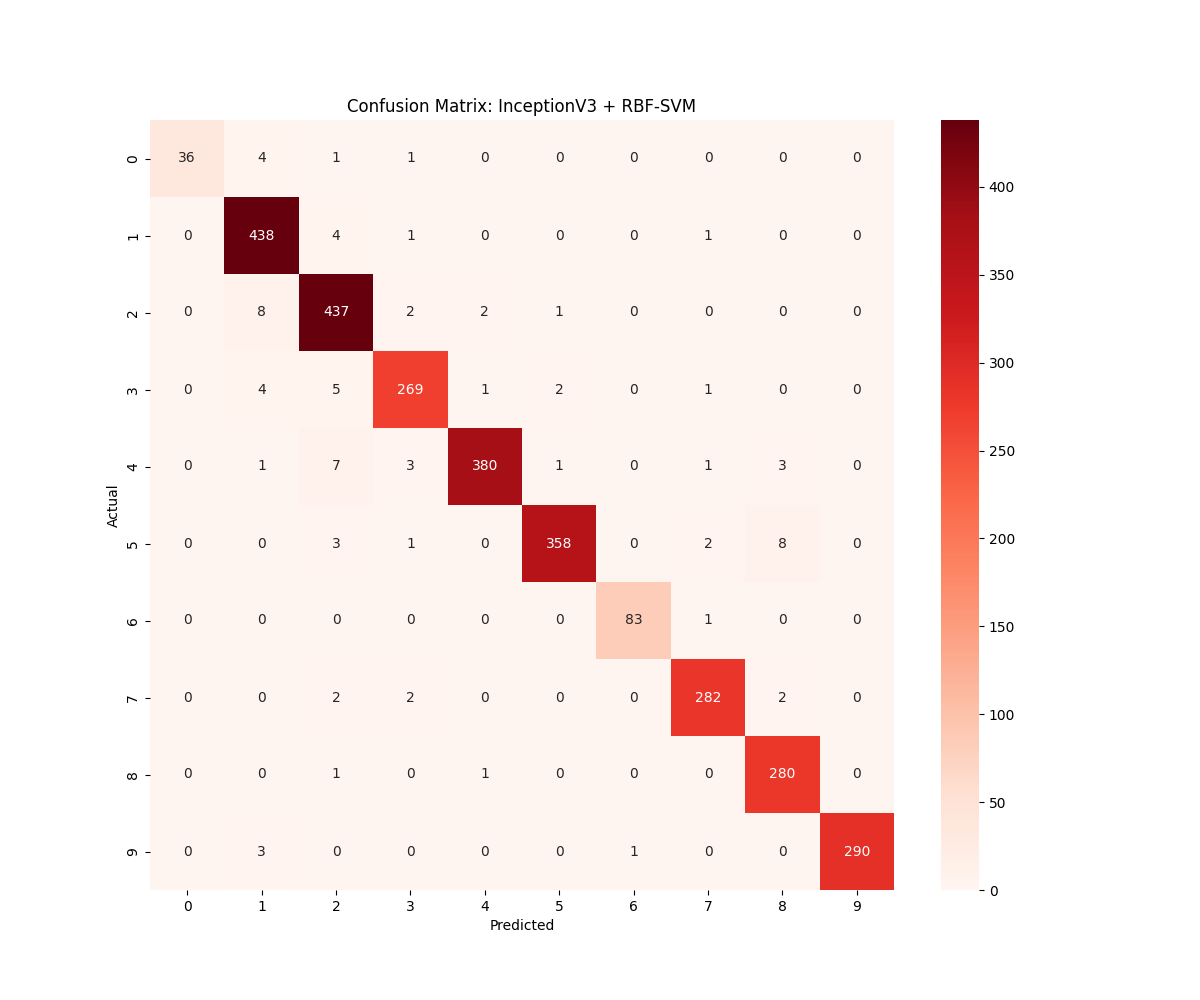
\includegraphics[width=\textwidth]{../reports/performance/inceptionv3_rbf_confusion_matrix.png}
        \caption{InceptionV3: RBF-SVM}
    \end{subfigure}
    \\[20pt]
    \begin{subfigure}[b]{0.48\textwidth}
        \centering
        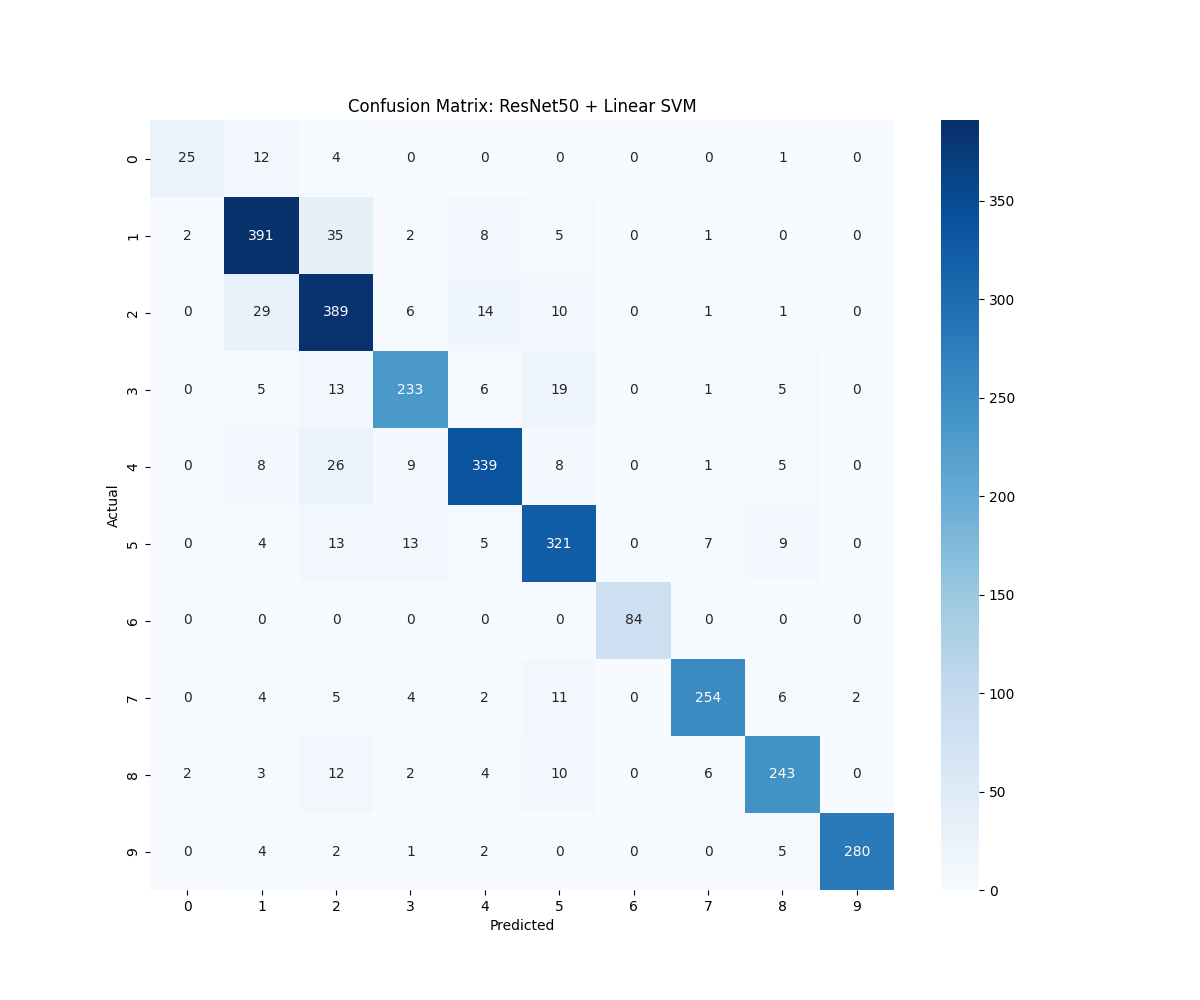
\includegraphics[width=\textwidth]{../reports/performance/resnet50_confusion_matrix.png}
        \caption{ResNet50: SGD-SVM}
    \end{subfigure}
    \hfill
    \begin{subfigure}[b]{0.48\textwidth}
        \centering
        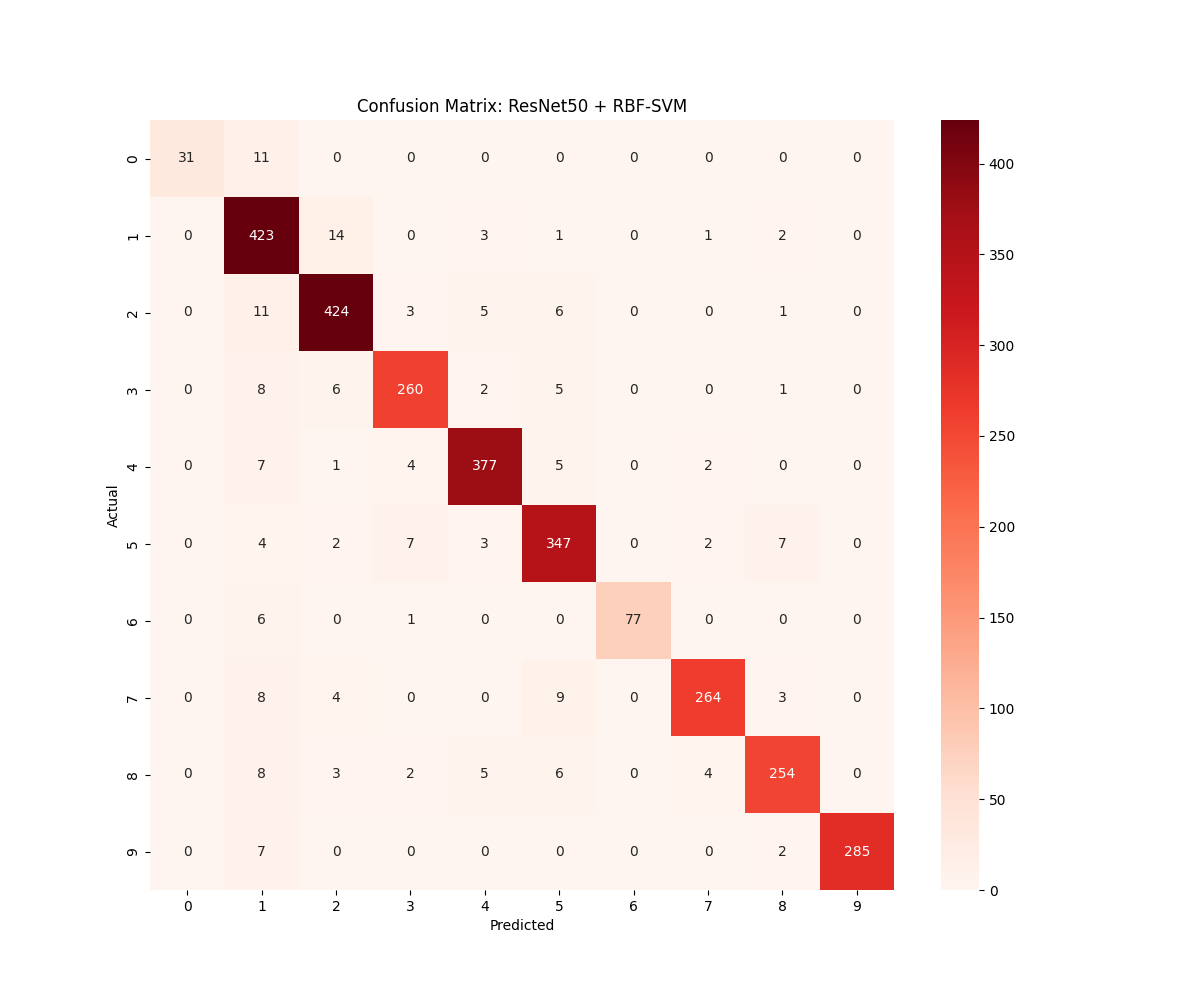
\includegraphics[width=\textwidth]{../reports/performance/resnet50_rbf_confusion_matrix.png}
        \caption{ResNet50: RBF-SVM}
    \end{subfigure}
    \caption{Confusion Matrix comparison for both architectures. The non-linear RBF kernel significantly clears the off-diagonal noise observed in the linear SGD models.}
    \label{fig:cm_comparison}
\end{figure}

The error analysis reveals that most misclassifications in the linear model occur within the speed limit sign family (e.g., confusing Class 2 with Class 1). However, the \textbf{RBF-SVM} significantly reduces these errors by finding more complex hyperplanes to separate these closely related feature clusters.

\section{Failure Case Analysis}
Despite the high accuracy achieved, a detailed inspection of the remaining misclassified samples (~270 cases across both models) reveals systematic patterns. Figure \ref{fig:failure_samples} illustrates representative failures from both ResNet50 and InceptionV3 pipelines.

\begin{figure}[H]
    \centering
    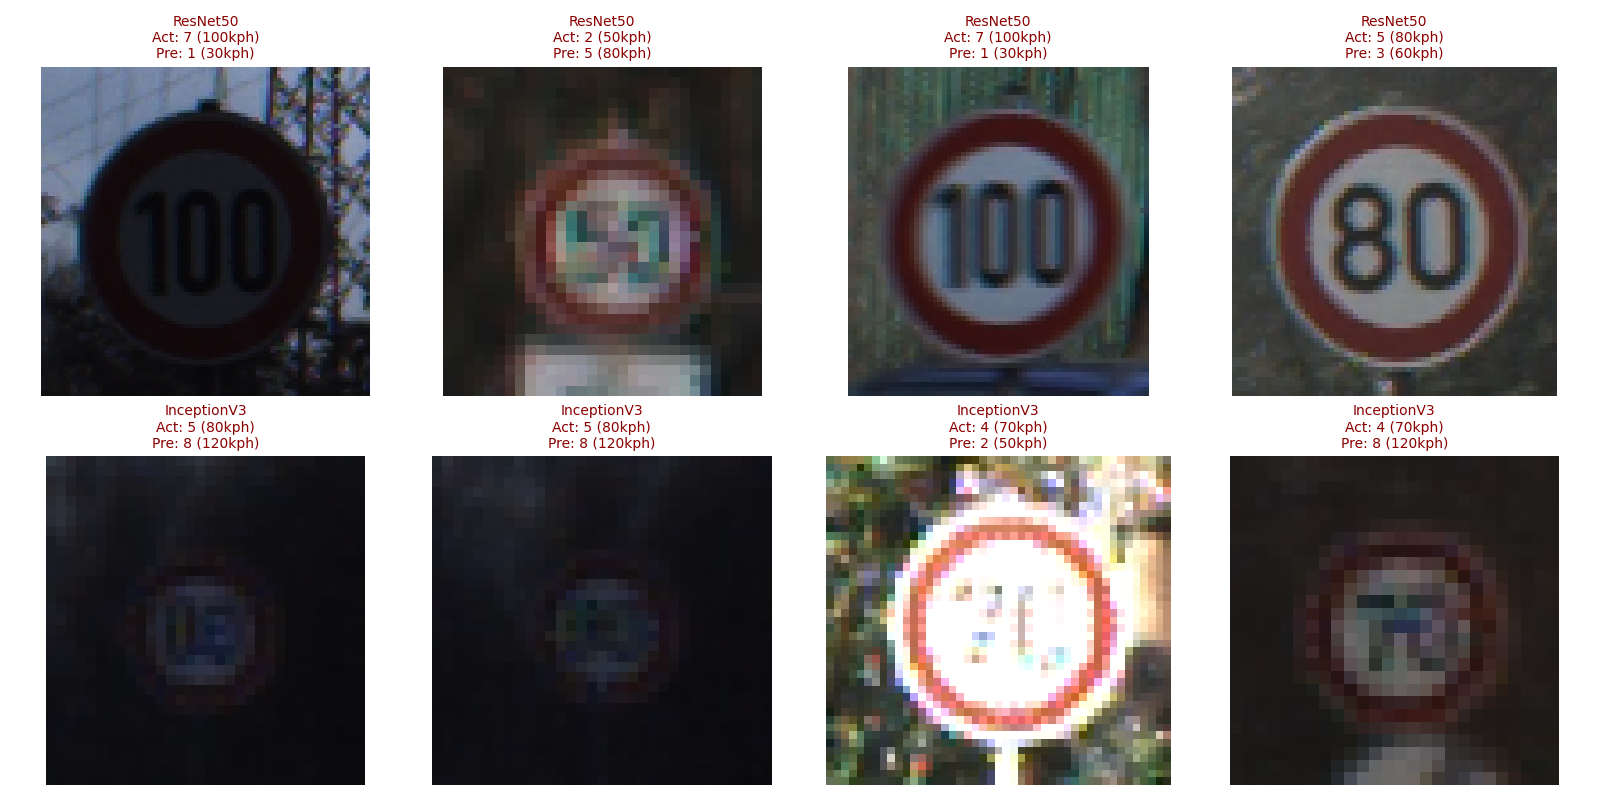
\includegraphics[width=0.95\textwidth]{../reports/performance/misclassified_samples.png}
    \caption{Representative Failure Cases. (A) Actual Label, (P) Predicted Label. Most errors involve visually similar digits (30 vs 50 km/h) or challenging environmental conditions.}
    \label{fig:failure_samples}
\end{figure}

The primary causes of failure can be categorized as follows:
\begin{enumerate}
    \item \textbf{High-InterClass Similarity:} The most frequent error pairs are 30 km/h (Class 1) vs. 50 km/h (Class 2) and 80 km/h (Class 5) vs. 120 km/h (Class 8). These signs differ only by a few central pixels representing the digits, which may be lost due to low resolution or blur.
    \item \textbf{Challenging Environmental Conditions:} Many failure cases occur in samples with extreme motion blur, heavy occlusion by roadside vegetation, or extremely low contrast caused by shadows. In these scenarios, even the deep feature extractors struggle to capture the distinguishing characteristics of the signs.
    \item \textbf{Data Imbalance Effects:} Class 0 (20 km/h) had the lowest recall, often being confused with Class 1 (30 km/h). This suggests that for minority classes with fewer training samples, the RBF kernel boundaries may still be slightly biased toward more frequent classes.
\end{enumerate}

\section{Discussion}
The consistent improvement provided by the RBF kernel (+6-9\% Accuracy) confirms the importance of addressing non-linear structures in deep feature manifolds. While InceptionV3 outperformed ResNet50 in peak accuracy, both architectures proved to be excellent feature extractors, transforming raw pixels into well-separated clusters that the SVM could effectively classify. The final 97.24\% accuracy meets the requirements for a reliable traffic sign recognition component in autonomous driving research contexts.
